
% Réalisé par: Mohand  Mamma et Clement fabre  
%Présenté le 20 Novembre  2014 



\documentclass[handout]{beamer}
\usepackage{pgfpages}
\usetheme{Warsaw}

\usepackage[utf8]{inputenc}
\usepackage{graphicx}
\graphicspath{ {Image/} }

\title{Les langages d'assemblage ou assembleur.}

\subtitle{}

\author{Mamma Mohand \and Fabre Clement }

\institute[UM2]
{
  Département informatique
  Université de Montpellier 2
}

\date{TCCP, 2014}

\subject{Les languages d'assemblage ou assembleur}

\AtBeginSubsection[]
{
  \begin{frame}<beamer>{Sommaire}
    \tableofcontents[currentsection,currentsubsection]
  \end{frame}
}

% Début du document
\begin{document}

\begin{frame}
  \titlepage
\end{frame}

\begin{frame}{Sommaire}
  \tableofcontents
\end{frame}

\section{Introduction}
\begin{frame}{Introduction}
Un langage assembleur (ou d'assemblage) est un langage de bas niveau qui représente le langage machine sous une forme lisible par un humain. Le terme assembleur est aussi utilisé pour désigner le programme qui traduit le langage assembleur pour le convertir en langage machine.
\end{frame}

\section{Histoire}
\begin{frame}{Histoire}
\begin{itemize}
\item En 1949, les programmes du premier calculateur à programmes enregistrés étaient rédigés en utilisant des mnémoniques alphabétiques. La traduction était alors faite à la main par les programmeurs.
\item Le premier programme assembleur a été écrit par Nathaniel Rochester en 1954.
\item Les langages assembleur ont éliminé une grande partie des erreurs commises par les programmeurs. On a donc commencé à les utiliser dans toutes sortes de programme.
\end{itemize}
\end{frame}
 
   
\section{Principes de programmation en Assembleur} 
\subsection{Programmer en assembleur} 
\begin{frame}{Programmer en assembleur}
 \begin{figure}
  	\centering
   	 \includegraphics[scale=0.35]{Programmer.png}
    	\caption{Programmer en assembleur.}
    
    \end{figure}   
\end{frame}


\begin{frame}{Petit Rappel}{Processeur}
    \begin{block}{Definition}
       Composant de l'ordinateur qui  exécute les instructions machines des programmes informatique.
    \end{block}
    \pause
  Les parties essentielles  d'un processeur:
    \begin{itemize}{}
       	\item Unité arithmétique et logique.
	\item Unité de controle.
	\item Les registre.
    \end{itemize}
\end{frame}

\begin{frame}{Petit rappel}{Registre} 
 \begin{block}{Definition}
      C'est la mémoire la plus rapide d'un ordinateur .
    \end{block}
L' architecture externe du processeur définit un ensemble de registre. \newline{}
Ces registres sont accessible par leur jeu  d’instruction .  
\end{frame}

\begin{frame}{Petit rappel}{Registre}
    \begin{figure}
    \centering
    \includegraphics[scale=0.23]{Registre.png}
    \caption{Différents registres existants.}
    \label{fig:Registre}
    \end{figure}
\end{frame}

\subsection{La syntaxe de l'assembleur} 

\begin{frame}{Section}
     Un programme  en assembleur  peut etre  divisé en 3 sections: 
 
   \begin{itemize}
 	   \item .txt :contient les instructions et les constantes du programme.
 	   \item .data  :décrit comment allouer l'espace mémoire.
   	   \item .bss :contient les variables non initialisées. 
    \end{itemize}
 

\end{frame}

\begin{frame}{Declaration}
\begin{block}{}
 Peuvent prendre quatre formats .\newline{}
 Se  termine par un saut  a la ligne ou un ;. 
\end {block}
Illustration: 

 \begin{figure}
    \centering
    \includegraphics[scale=0.65]{code00.png}
	 \caption{Example de declaration.}
    \end{figure}
 \begin{block}{Important}
	le symbole « . » : 	peut etre utilisé  comme référence a une adresse lors de l'assemblage.\newline{}
 \end {block}


\end{frame}

\begin{frame}{Symbole}
     Séquences  de caractères choisie parmi :
    \vspace{\baselineskip}
    \begin{itemize}
    \item{Les lettres de l'alphabet.}
    \item{Les  chiffres décimaux.}
    \item{Les  caractères :.\$}
    \end{itemize}
\end{frame}

\begin{frame}{Symbole}
     à connaitre :
    \vspace{\baselineskip}
    \begin{itemize}
    \item{Les Symboles ne doivent jamais  commencer par un  chiffres.}
    \item{Un symbole doit commencer en  début de ligne}
    \item{La  casse est significatives.}
    \item{Un symbole  suivie de : est   appelé  étiquette.}
    
\begin{block}{Important} 
Le symbole spécial « . » peut être utilisé comme une référence à une adresse au moment de l'assemblage.
\end{block}
    \end{itemize}
Example:\newline{}
len = . - msg 
\end{frame}

\begin{frame}{Symbole}{Symbole local }
    
         Le GNU propose 10 symbole locaux [0,1,........ ,9].
 	\begin{block}{Annotation}
    		Nb:se réfere au dernier symbole  N défini	 \newline{}
		Nf:se refére au premier symbole N suivant

\end{block}
Exemple: 
 \begin{figure}
    \centering
    \includegraphics[scale=0.55]{Code1.png}
	
    \end{figure}

\end{frame}

\begin{frame}{Nombre entier}

 \begin{figure}
    \centering
    \includegraphics[scale=0.25]{Nombreentier.png}
    \caption{Representation  des constantes.}
    \label{fig:Types Constante}
    \end{figure}
\end{frame}

\begin{frame}{Chaine de caractéres}
   \begin{block}{Definition}
	C'est une séquence de caractères écrite entre guillemets.\newline{}
	 Elle représente un tableau contigu d'octets en mémoire. 
	\end{block} 
Example de Code: \newline{} 
msg :               .asciz "Hello, World !\n"
\end{frame}


\subsection{Instruction}

\begin{frame}{Instruction}
   \begin{block}{Definition}
	L'élement clé de l'ordinateur car c'est elle qui permet de spécifier au processeur l'action à effectuer.\newline{}
	Toutes les instructions sont stockées en mémoire.
	\end{block} 
 \begin{figure}
    \centering
    \includegraphics[scale=0.27]{Instruction.png}
    \caption{Une Instruction.}
    \label{fig:Une instruction}
    \end{figure}


\end{frame}


\begin{frame}{Instruction}{Instruction d'affectation}
   \begin{block}{Definition}
	Permettent de faire des transferts de données entre les registres et la mémoire.
	\end{block} 
 \begin{figure}
    \centering
    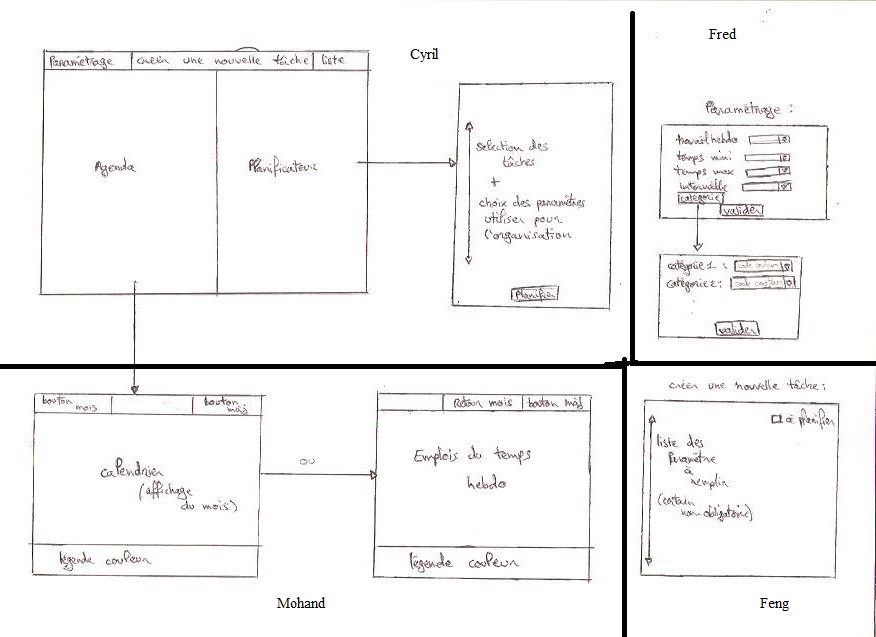
\includegraphics[scale=0.27]{Image.jpg}
    \caption{Une Instruction d'affectation.}
    \label{fig:Une instruction d'affectation.}
    \end{figure}

\end{frame}
\begin{frame}{Instruction}{Instruction arithmétique et logique}
    \begin{figure}
    \centering
    \includegraphics[scale=0.27]{Diagramme2.png}
    \caption{Instruction arithémitique et logique.}
    \label{fig:Instruction}
    \end{figure}
	
\end{frame}

\begin{frame}{Instruction}{Liste d'instruction}
    \begin{figure}
    \centering
    \includegraphics[scale=0.45]{Tableau.png}
    \caption{Liste d'instruction.}
    \label{fig:Instruction}
    \end{figure}
	
\end{frame}
\subsection{Exemple de code} 
\begin{frame}{Exemple de code}

\begin{figure}
  	\centering
   	 \includegraphics[scale=0.65]{C1.png}
    	\caption{Programmer en assembleur.}
    
    \end{figure}   
\end{frame}

\begin{frame}{Exemple de code}

\begin{figure}
  	\centering
   	 \includegraphics[scale=0.65]{C2.png}
    	\caption{Programmer en assembleur.}
    
    \end{figure}   
\end{frame}
\subsection{Assembleur et langages de haut niveau}
\begin{frame}{Assembleur et langages de haut niveau}
\begin{itemize} 

	\item Certain Language permettent d'ajouter du code ASM dans la source d'un programme.
	\item Cette technique est utilisé principalement par soucis de rapidité.

\end{itemize} 
Example  en  C++: 

    \begin{figure}
    \centering
    \includegraphics[scale=0.59]{C4.png}
    \caption{Liste d'instruction.}
    \label{fig:Instruction}
    \end{figure}
	
\end{frame}
\section{Usage}
\subsection{Souci d'efficacité} 
\begin{frame}{Souci d'efficacité}
Dans beaucoup de cas, des compilateurs-optimiseurs peuvent transformer du langage de haut niveau en un code qui tourne aussi efficacement qu'un code assembleur écrit à la main par un très bon programmeur.

\begin{block}{Manuel FORTRAN (1956) :}
\it
Object programs produced by Fortran will be nearly as efficient as those written by good programmers
\end{block}
\end{frame}

\subsection{Cas d'utilisation} 
\begin{frame}{Cas d'utilisation}

\begin{itemize}
\item Calculs complexes
\item Routines (ou drivers)
\item Tâches effectuées dans l'espace mémoire du système d'exploitation
\item Debogage et profilage
\item Micro-contrôleurs limités en ressources
\end{itemize}

\end{frame}



\section{Conclusion}
\subsection*{Conclusion}
\begin{frame}{Conclusion}
La programmation en assembleur est beaucoup plus longue, plus délicate et donc plus coûteuse que la programmation en langage de haut niveau. Il est donc conseillé de ne l'utiliser que si on peut pas faire autrement.    
\end{frame}

\begin{frame}{}
    \centering
    \textbf{Merci de votre attention}
\end{frame}

\end{document}


